% sections/10_qa.tex

\begin{frame}[plain]
  \centering
  \vfill
  \begin{beamercolorbox}[sep=12pt,center,rounded=true,shadow=true]{palette primary}
    \usebeamerfont{title}\Huge Questions? \\
    \vspace{0.3cm}
    \usebeamerfont{title}\Large Obrigado! \raisebox{-1pt}{\(\mathbf{\ddot{\smile}}\)}
  \end{beamercolorbox}
  \vfill
  
  \begin{columns}[onlytextwidth, T]
    \column{0.5\textwidth}
      \centering
      \small \textbf{Distributed Work} \\
      \vspace{0.2cm}
      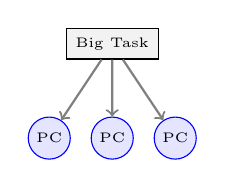
\begin{tikzpicture}[scale=0.8]
        % Top task
        \node[draw, fill=gray!10] (task) at (1,1.5) {\tiny Big Task};
        
        % Three small PC nodes
        \node[circle, draw=blue, fill=blue!10, inner sep=2pt] (p1) at (0,0) {\tiny PC};
        \node[circle, draw=blue, fill=blue!10, inner sep=2pt] (p2) at (1,0) {\tiny PC};
        \node[circle, draw=blue, fill=blue!10, inner sep=2pt] (p3) at (2,0) {\tiny PC};
        
        % Arrows showing the split
        \draw[->, thick, gray] (task) -- (p1);
        \draw[->, thick, gray] (task) -- (p2);
        \draw[->, thick, gray] (task) -- (p3);
      \end{tikzpicture}
      
    \column{0.5\textwidth}
      \centering
      \small \textbf{Speed Comparison} \\
      \vspace{0.2cm}
      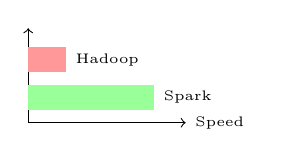
\begin{tikzpicture}[scale=0.8]
        % Simple Bar Chart
        \draw[->] (0,0) -- (2.5,0) node[right] {\tiny Speed};
        \draw[->] (0,0) -- (0,1.5);
        
        % Hadoop Bar (Short)
        \fill[red!40] (0,0.8) rectangle (0.6,1.2);
        \node[right] at (0.6,1.0) {\tiny Hadoop};
        
        % Spark Bar (Long)
        \fill[green!40] (0,0.2) rectangle (2.0,0.6);
        \node[right] at (2.0,0.4) {\tiny Spark};
      \end{tikzpicture}
  \end{columns}

  \vfill
  \textbf{\MyAuthor} \\
  \small \MyInstitute \\
  \vspace{0.2cm}
  \small \texttt{\MyEmail}
  \vfill
\end{frame}
